\section{About Data Integrity}
Storing cultural heritage in digital archives offers malicious actors the possibility to manipulate the data and possibly forge history. Recent digital technologies make data manipulation more efficient, less costly, and more exact and there is a long history of forging history. 
In 1920 a photography was taken of Vladimir Lenin atop a platform speaking to a crowd. In the original photo, see Figure \ref{fig:f1}, Lenin's comrade Leon Trotsky can be seen standing beside the platform on Lenin's left side. When power struggles within the revolution forced Trotsky out of the party 7 years later, he was retouched out of the picture, see Figure \ref{fig:f2}, using paint, razors and airbrushes. Soviet photo artists altered the historical record by literally removing Trotsky from the pictures \cite[3]{hofer2005digital}.

\begin{figure}[t]%
    \centering
    \begin{subfigure}{6cm}
    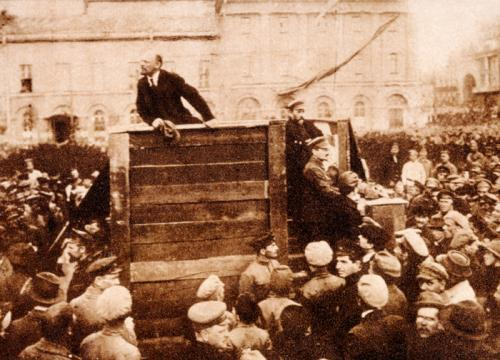
\includegraphics[width=\linewidth]{graphics/trotzki1.jpg}
    \caption{Original}\label{fig:f1}
    \end{subfigure}
    \qquad
    \begin{subfigure}{6cm}
    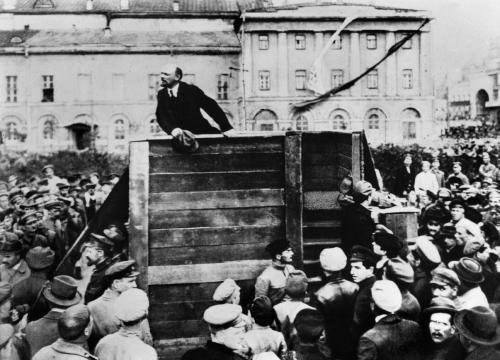
\includegraphics[width=\linewidth]{graphics/trotzki2.jpg}
    \caption{Retouched}
    \label{fig:f2}
    \end{subfigure}
    \caption{Catalog Images}
\end{figure}

Digital archives must earn the trust of current and future digital creators by developing a robust infrastructure and long-term preservation plans to demonstrate that the archive and its staff are trustworthy stewards of the digital materials in their care \cite[37]{kirschenbaum2010digital}. Digital objects can be corrupted easily, with or without fraudulent intent, and even without intent at all. Data corruption is usually detected by comparing cryptographic hashes, so-called fixity information, at different time intervals \cite[1]{de2014checking}. The object is seen as uncorrupted if the hash values are identical, since the smallest change to the object would alter the newly computed hash value immensely. 

\section{Research Problem}
Although generating fixity information (e.g., MD5, SHA256) is relatively easy, managing that information over time is harder \cite[35]{kirschenbaum2010digital}. Consider that if an actor can change the fixity information, the actor can also tamper the underlying data. Fixity information is usually stored in databases; object metadata records or alongside content, whereas this thesis utilizes the blockchain as a storage medium.
It is shown, that the Ethereum blockchain is suited for storage of metadata, such as provenance data or fixity information \cite[1]{collomosse2018archangel}.

Collomosse et al. (2018) and Sigwart et. al (2020) have shown that the Ethereum blockchain, developed by Buterin et. al (2013), can indeed be utilized to ensure data integrity, but there is a problem with that: the operation cost. The cost of storing a SHA256 values on the Ethereum blockchain is about \$8, which means the operation cost for an ingest of 10,000 objects costs about \$80,000.

\section{Research Goal}
This thesis proposes a way to reduce the operational cost of a blockchain-based fixity information storage by applying a pool testing strategy in which several digital objects are combined in a pool to form a hash list. The idea for this approach stems from the ongoing pandemic, in which the test capacities also must be used optimally.
\begin{quote}
Pool testing strategies build on testing a pooled sample from several patients: if the results from the pool test are negative, all patients in the pooled sample are declared not to have COVID-19; if the results of the pool are positive, each patient sample is tested individually. The pooled testing strategy is appealing, particularly when test availability is limited \cite[1]{cherif2020simulation}.
\end{quote}
This paradigm will be utilized in this thesis where the test specimen are cryptographic hashes, and the pool is hash list. With pooled testing, the goal is to reduce the amount of transactions, and therefore the cost by at least 50\%.

\section{Research Questions}
Based on the problem described above, the following research questions arise:

\textit{RQ1 What is the optimal pool size based on the change rates of digital objects in the archive regarding cost and efficiency?}

\textit{RQ2 To what extent can pooled testing increase the efficiency and reduce cost for a fixity information storage service on the Ethereum blockchain?}

\textit{RQ3 Given that metadata has a higher change rate, what effect has the split of metadata and objects on the operation cost?}

\section{Research Approach}
\label{sec:approach}
This work will follow the principles of Design Science Research, from \cite{hevner2007three}. The artifact is designed based on a literature review of the following main topics: Diplomatics of Digital Records, Ethereum Blockchain and Pooled testing.

The application environment is a digital archive that manages any kind of data, such as images or text. Data is referred to in the archive as an Information Object (IO) and each object is provided with metadata to guarantee readability in the future, as described in the OAIS reference model. I assume that the data integrity must be ensured on ingest where a cryptographic hash value of the information object is computed and stored on the blockchain. The "location" of the fixity information on the blockchain is stored in the Preservation Description Information (PDI) in the form of a unique transaction hash, see Figure \ref{fig:oais-fixity}. 

\begin{figure}[t]
  \centering
  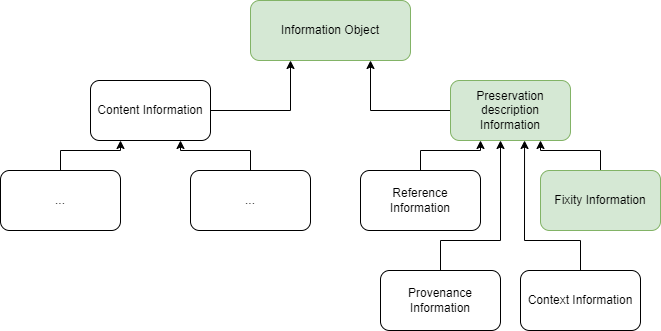
\includegraphics[width=0.7\textwidth]{oais.png}
  \caption{The transaction hash, used to retrieve data from the blockchain, is stored in the fixity information of the PDI of an information object \cite[7]{lee2010open}.}
  \label{fig:oais-fixity}
\end{figure}

The \textit{Artifact} is a combination of decentralized application on the Ethereum blockchain and a local pool structure in the archive. The smart contract exposes functions for managing cryptographic hashes of pools.
The artifact must provide the following functionalities:
\begin{itemize}
  \item Create, Read, Update SHA256 values of pools.
  \item Must hold a reference (ID) for the respective pool in the archive.
  \item Must be tamperproof for unauthorized calls.
\end{itemize}
The smart contract complements the local pool structure in the archive where fixity information of certain object pools may be requested on any given time. The artifact should reduce the amount of operations needed to ensure the integrity of 10,000 objects from ingest to retrieval process by at least 50\%.

\section{Structure of the work}
The remainder of this work is structured as follows:
\begin{enumerate}[label=\textbf{\arabic*})]
  \setcounter{enumi}{1}
  \item \textbf{Related Work} presents the state of the art of projects that utilize the Ethereum blockchain as a storage medium for metadata
  \item \textbf{Diplomatics of Digital Records} gives an overview of the abstract concept of trust in digital archives
  \item \textbf{Ethereum Blockchain} gives an overview of the concepts and functions of the Ethereum ecosystem
  \item \textbf{Fixity Storage} contains an introduction to fixity information and how to handle it, this chapter also contains the implementation and deployment of the fixity storage utilized in this work
  \item The \textbf{Evaluation} chapter contains the answers to the research questions 
  \item I interpret and explain the results in the \textbf{Discussion} chapter
  \item \textbf{Conclusion} suggests future work and my contribution to the digital preservation research field
\end{enumerate}